\documentclass[a4paper, 11pt]{beamer}

\mode<presentation>
{
  \usetheme{Madrid}
  % or ...
  %\usetheme{Darmstadt}
  \usefonttheme[onlylarge]{structurebold}
  \setbeamerfont*{frametitle}{size=\normalsize,series=\bfseries}
  \setbeamertemplate{navigation symbols}{}


  \setbeamercovered{transparent}
  % or whatever (possibly just delete it)
}

\usepackage{polski}
\usepackage[utf8]{inputenc}
\usepackage{times}
\usepackage[T1]{fontenc}
\usepackage{amsmath}

\title[Model rynku Arrowa-Hurwicza]
{
  Równowaga rynkowa\\
  Model rynku Arrowa-Hurwicza
}

\author[Kruszewski, Paulukanis, Sochoń]
{
  Mateusz Kruszewski  \and
  Adam Paulukanis     \and
  Paweł Sochoń
}

\institute[UwB]
{
  Uniwersytet w Białymstoku
}

\date[Białystok, 2012]
{
  Białystok, 2012
}

\AtBeginSection[]
{
  \begin{frame}<beamer>{Outline}
    \tableofcontents[currentsection,currentsubsection]
  \end{frame}
}

\begin{document}

  \begin{frame}
    \titlepage
  \end{frame}

  \begin{frame}{Outline}
    \tableofcontents
  \end{frame}


  \section{Równowaga rynkowa}
    \subsection{Wstęp}

      \begin{frame}{Wstęp}
	\begin{columns}[c]
	  \column{.4\textwidth}
	    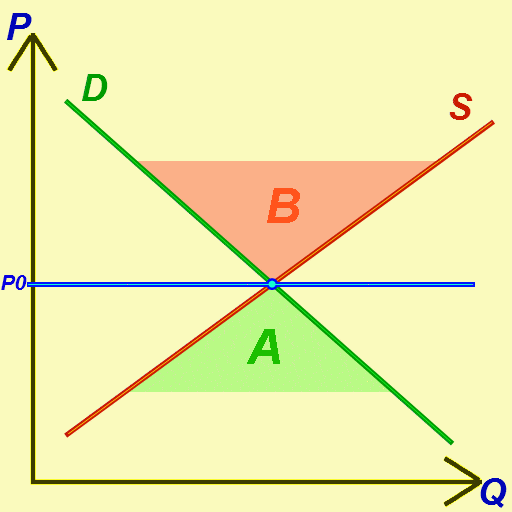
\includegraphics[height=4.5cm]{Price_of_market_balance.png}

	  \column{.6\textwidth}
	    Nie interesuje nas pochodzenie dostarczanych na rynek towarów, ani
	    mechanizm alokacji czynników produkcji. Zakładamy, że każdy postępuje
	    racjonalnie, a gospodarka jest zdecentralizowana. 
      	\end{columns}
      \end{frame}

    \subsection{Model rynku wg. Arrowa-Hurwicza}

      \begin{frame}{Model rynku wg. Arrowa-Hurwicza}
	\begin{center}
	  Model ten opracowali Leonid Hurwicz i Kenneth Joseph Arrow.
	\end{center}
  
	\begin{columns}[c]
	  \column{.5\textwidth}
	    Opisuje on ludzi (\textit{kupców}) sprzedających i kupujących towary przy
	    założeniach:

	    \vskip10pt
	    \begin{itemize}
	      \item kupcy maksymalizują swoje indywidualne korzyści,
	      \item popyt na towary jest równy ich podaży.
	    \end{itemize}

	    \vskip20pt
	    Na rynek przybywa $m$ kupców, przynosząc $n$ rodzajów towarów.

	  \column{.4\textwidth}
	    \begin{center}
	      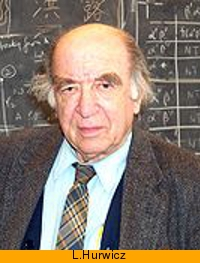
\includegraphics[height=3cm,width=2.5cm]{200px-Leonid_Hurwicz_x.jpg}\\
	      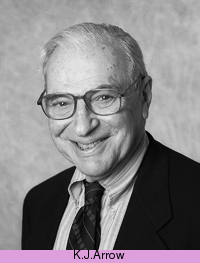
\includegraphics[height=3cm,width=2.5cm]{Kenneth_Arrow_x.jpg}

	    \end{center}
	\end{columns}
	
      \end{frame}

      \begin{frame}{Model rynku wg. Arrowa-Hurwicza c.d.}
	Oznaczenia:

	\begin{itemize}
	  \item $y^k=(y_1^k, \ldots, y_n^k)$ -- koszyk towarów dostarczanych na
	  rynek przez $k$-tego kupca,

	  \item $x^k=(x_1^k, \ldots, x_n^k)$ -- koszyk towarów, które jest on
	  gotów nabyć,

	  \item $p=(p_1, \ldots, p_n)$ -- wektor cen towarów,

	  \item $X^k=R_{+}^n$ -- przestrzeń towarów $k$-tego kupca,
	\end{itemize}

	gdzie: $k=1, \ldots, m$.

      \end{frame}

      \begin{frame}{Model rynku wg. Arrowa-Hurwicza c.d.}
	Zakładamy, że
	\[ <p, x^k> \leq <p,y^k>, \]
	czyli wartość nabywanego przez kupca $k$ koszyka towarów nie przekracza
	wartości towarów przez niego sprzedawanych.

	\vskip10pt
	Ponadto zakładamy, że kupcy nie dysponują żadnymi innymi dochodami poza
	tymi, które uzyskują ze sprzedaży swoich zapasów towarów.

	\vskip10pt
	Kupiec ma pewne preferencje, które opisujemy przy użyciu funkcji
	użyteczności $u^k (k=1, \ldots, m)$.

      \end{frame}

    \subsection{$k$-ty kupiec wybiera koszyk $x^k$}

      \begin{frame}{Wykres}
	\begin{center}
	  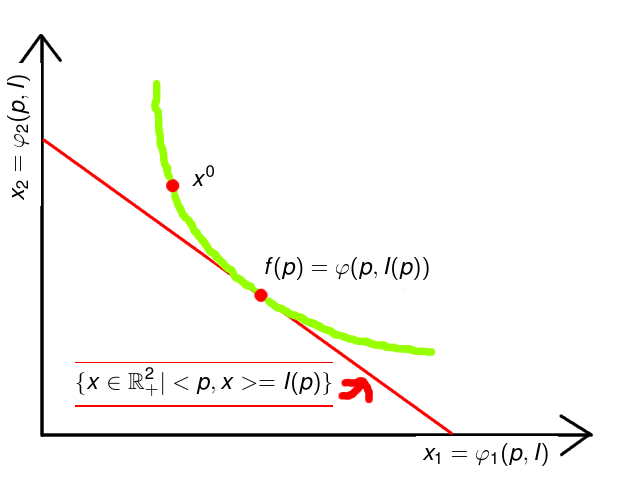
\includegraphics[height=8cm]{wykres1.png}
	\end{center}
      \end{frame}

      \begin{frame}{$k$-ty kupiec wybiera koszyk $x^k$}

	\begin{columns}
	  \column{.55\textwidth}
	    Jeżeli funkcje $u^k$ są ciągłe, silnie wklęsłe i rosnące
	    na $\mathbb{R}^n_{+}$, to jest to standardowy warunek, przy którym
	    rozwiązaniem \textit{Zadania} jest ciągła na $\text{int} \,
	    \mathbb{R}^{n+1}_{+}$  $x^k$ funkcja cen $p$ i dochodu $<p, y^k> = I^k$,
	    czyli
	    \[ x^k = \varphi^k (p, I^k), \]

	  \column{.45\textwidth}
	    \begin{block}{\textit{Zadanie}}
	      \begin{tabular}{rl}
		fc: & $u^k(x) \to \text{max}$\\
		wo: & $\left\{\begin{array}{l}
				  <p, x> \leq <p, y^k>\\ 
				  x \geq 0 
			      \end{array}
		       \right.$
	      \end{tabular}
	    \end{block}
       \end{columns}

    \vskip3pt
          gdzie
     \[ \varphi^k (p, I^k) = \arg \max_{\begin{array}{c} <p, x> \leq I^k\\ x
     \geq 0 \end{array}} u^k(x). \]

     Dla wygody zamiast $x^k$ będziemy pisać $$f^k(p) = \varphi^k (p, I^k) =
     \varphi^k (p, <p, y^k>).$$

    \end{frame}

    \subsection{Wektor nadmiernego (nadwyżkowego) popytu na towar}

      \begin{frame}{Wektor nadmiernego (nadwyżkowego) popytu na towar}
	\begin{block}{Definicja: (\textit{popyt} minus \textit{podaż})}
	  $$z(p) = \sum_{k=1}^m x^k - \sum_{k=1}^m y^k = \sum_{k=1}^m f^k (p) -
	  \sum_{m=1}^m y^k$$
	\end{block}

	\begin{description}
	  
	  \item[$z_i (p) > 0$] oznacza nadwyżkę popytu nad podażą towaru $i$,

	  \item[$z_i (p) < 0$] oznacza nadmiar podaży nad popytem towaru $i$.

	\end{description}
	
	\begin{center}
	\alert{,,Popyt na towar oferowany za darmo\\ zawsze przekracza
	jego podaż.''}
	\end{center}
	\[ \forall_i (p_i=0 \rightarrow z_i (p) > 0). \]

      \end{frame}

    \subsection{Rynek w równowadze}

      \begin{frame}{Rynek w równowadze}
	\begin{block}{Definicja: $z(\overline{p}) = 0$}
	  Mówimy, że \textbf{rynek jest w równowadze}, jeżeli ustaliły się na
	  nim ceny $\overline{p} > 0$, przy których wektor nadmiernego popytu
	  spełnia warunek
	  \[ z(\overline{p}) = 0. \]
	\end{block}

	Wektor $\overline{p}$ nazywamy \textbf{wektorem cen równowagi}.
    \end{frame}
    \subsection{Jeden dodatni wektor cen równowagi rynkowej}
      \begin{frame}{Jeden dodatni wektor cen równowagi rynkowej}
	Założenia:
	\begin{enumerate}
	  \item[(I)] Funkcje $f^k$ są ciągłe i różniczkowalne na
	  $\mathbb{R}^n_{+} \ \{0\}$,

	  \item[(II)] $\forall_i (p_i = 0 \rightarrow z_i (p) > 0$,

	  \item[(III)] Macierz funkcyjna $J(p) = (\frac{a}{b})_{(n, n)}$
	  uzupełnić BRAKUJE
	\end{enumerate}

	\begin{block}{Model Arrowa-Hurwicza}
	  Istnieje jeden dodatni wektor cen równowagi rynkowej określony z
	  dokładnością do struktury.
	\end{block}
      \end{frame}

  \section{Przykład}
    \subsection{Przykład 1}

  \section*{Koniec}
    \begin{frame}
      \begin{center}
	Dziękujemy za uwagę.
      \end{center}
    \end{frame}

\end{document}
